\documentclass[11pt,letterpaper]{article}
\usepackage[lmargin=1in,rmargin=1in,tmargin=1in,bmargin=1in]{geometry}
\usepackage{../style/homework}
\usepackage{../style/commands}
\setbool{quotetype}{false} % True: Side; False: Under
\setbool{hideans}{false} % Student: True; Instructor: False

% -------------------
% Content
% -------------------
\begin{document}

\homework{7: Due 06/07}{Science is simply common sense at its best, that is, rigidly accurate in observation, and merciless to fallacy in logic.}{Thomas Huxley}

% Problem 1
\problem{10} Plot the quadratic function $y= 4 - (x + 6)^2$ as accurately as possible. Your sketch should include the vertex and axis of symmetry. 
	\[
	\fbox{
	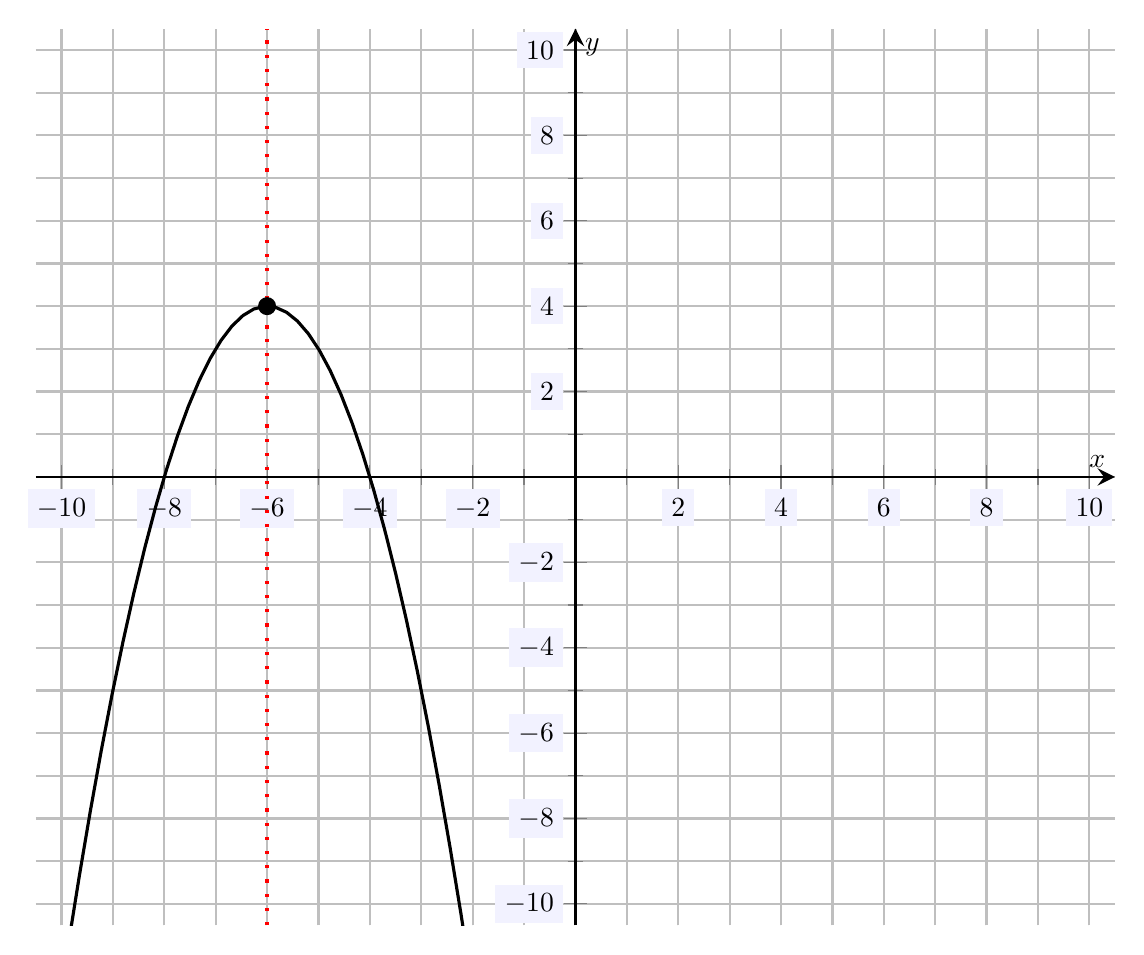
\begin{tikzpicture}[scale=2,every node/.style={scale=0.5}]
	\begin{axis}[
	grid=both,
	axis lines=middle,
	ticklabel style={fill=blue!5!white},
	xmin= -10.5, xmax=10.5,
	ymin= -10.5, ymax=10.5,
	xtick={-10,-8,-6,-4,-2,0,2,4,6,8,10},
	ytick={-10,-8,-6,-4,-2,0,2,4,6,8,10},
	minor tick = {-10,-9,...,10},
	xlabel=\(x\),ylabel=\(y\),
	]
	\addplot[red,dotted,line width= 0.02cm,domain= -10.5:10.5] ({-6},{x}); 
	\draw[fill=black] (-6,4) circle (0.05cm);
	\addplot[line width= 0.02cm,domain= -10.5:10.5,samples=100] ({x},{4 - (x + 6)^2}); 
	\end{axis}
	\end{tikzpicture}
	}
	\] \pspace

\sol We know that $y= 4 - (x + 6)^2= -(x + 6)^2 + 4= -\big(x - (-6) \big)^2 + 4$ is in vertex form, i.e. the form $y= a(x - P)^2 + Q$ with $a= -1$, $P= -6$, and $Q= 4$. Therefore, the vertex of $y= 4 - (x + 6)^2$ is $(-6, 4)$ and the axis of symmetry is $x= -6$. Because $a= -1 < 0$, the parabola opens downwards. This gives the sketch above. 



\newpage



% Problem 2
\problem{10} Find the vertex form of $f(x)= x^2 - 12x + 41$. Also, find the vertex and axis of symmetry of $f(x)$. \pspace

\sol The vertex form of a function $f(x)= ax^2 + bx + c$ is a form $y= a(x - P)^2 + Q$, where $(P, Q)$ is the vertex and $x= P$ is the axis of symmetry. We find the vertex form of $f(x)= x^2 - 12x + 41$ by completing the square: \pspace
	\[
	\begin{aligned}
	f(x)&= x^2 - 12x + 41 \\[0.3cm]
	&= x^2 - 12x + (12/2)^2 - (12/2)^2 + 41 \\[0.3cm]
	&= x^2 - 12x + 36 - 36 + 41 \\[0.3cm]
	&= (x^2 - 12x + 36) + (-36 + 41) \\[0.3cm]
	&= (x - 6)^2 + 5
	\end{aligned}
	\] \pspace
Therefore, $(6, 5)$ is the vertex and $x= 6$ is the axis of symmetry. \pspace

\begin{center} {\bfseries OR} \end{center}

The vertex form of a function $f(x)= ax^2 + bx + c$ is a form $y= a(x - P)^2 + Q$, where $(P, Q)$ is the vertex and $x= P$ is the axis of symmetry. We know the $x$-coordinate of the vertex is $x= -\frac{b}{2a}$. But we have $x= -\frac{b}{2a}= -\frac{-12}{2(1)}= \frac{12}{2}= 6$. The $y$-coordinate of the vertex is\dots \pspace
	\[
	f(6)= 6^2 - 12(6) + 41= 36 - 72 + 41= 5
	\] \pspace
Therefore, the vertex is $(6, 5)$. We know that $a= 1$. Then vertex form is $f(x)= 1(x - 6)^2 + 5= (x - 6)^2 + 5$ and the axis of symmetry is $x= 6$. 



\newpage



% Problem 3
\problem{10} Find the vertex and axis of symmetry of $g(x)= -3x^2 + 24x - 37$. \pspace

\sol The vertex form of a function $f(x)= ax^2 + bx + c$ is a form $y= a(x - P)^2 + Q$, where $(P, Q)$ is the vertex and $x= P$ is the axis of symmetry. We find the vertex form of $g(x)= -3x^2 + 24x - 37$ by completing the square: \pspace
	\[
	\begin{aligned}
	g(x)&= -3x^2 + 24x - 37 \\[0.3cm]
	&= -3 \left( x^2 - 8x + \dfrac{37}{3} \right) \\[0.3cm]
	&= -3 \left( x^2 - 8x + (-8/2)^2 - (-8/2)^2 + \dfrac{37}{3} \right) \\[0.3cm]
	&= -3 \left( x^2 - 8x + 16 - 16 + \dfrac{37}{3} \right) \\[0.3cm]
	&= -3 \left( (x^2 - 8x + 16) + \left( -16 + \dfrac{37}{3} \right) \right) \\[0.3cm]
	&= -3 \left( (x - 4)^2 + \left( -\dfrac{48}{3} + \dfrac{37}{3} \right) \right) \\[0.3cm]
	&= -3 \left( (x - 4)^2 - \dfrac{11}{3} \right) \\[0.3cm]
	&= -3(x - 4)^2 + 11
	\end{aligned}
	\] \pspace
Therefore, $(4, 11)$ is the vertex and $x= 4$ is the axis of symmetry. \pspace

\begin{center} {\bfseries OR} \end{center}

The vertex form of a function $f(x)= ax^2 + bx + c$ is a form $y= a(x - P)^2 + Q$, where $(P, Q)$ is the vertex and $x= P$ is the axis of symmetry. We know the $x$-coordinate of the vertex is $x= -\frac{b}{2a}$. But we have $x= -\frac{b}{2a}= -\frac{24}{2(-3)}= -\frac{24}{-6}= 4$. The $y$-coordinate of the vertex is\dots \pspace
	\[
	g(4)= -3(4^2) + 24(4) - 37= -3(16) + 96 - 37= -48 + 96 - 37= 11
	\] \pspace
Therefore, the vertex is $(4, 11)$. We know that $a= -3$. Then vertex form is $g(x)= -3(x - 4)^2 + 11$ and the axis of symmetry is $x= 6$. 



\newpage



% Problem 4
\problem{10} Consider the quadratic function $h(x)= 4x^2 - 12x + 6$.
        \begin{enumerate}[(a)]
        \item Determine if the parabola opens upwards or downwards.
        \item Is the parabola convex or concave?
        \item Does the parabola have a maximum or minimum? 
        \item Find the vertex and axis of symmetry. 
        \item Find the maximum/minimum value of $h(x)$. 
        \end{enumerate} \pspace

\sol
\begin{enumerate}[(a)]
\item The function $h(x)= 4x^2 - 12x + 6$ is of the form $ax^2 + bx + c$. Because $a= 4 > 0$, we know that the parabola opens upwards. \pspace

\item The function $h(x)= 4x^2 - 12x + 6$ is of the form $ax^2 + bx + c$. Because $a= 4 > 0$, we know that the parabola is convex.\pspace

\item The function $h(x)= 4x^2 - 12x + 6$ is of the form $ax^2 + bx + c$. Because $a= 4 > 0$, we know that the parabola opens upwards or is convex. Therefore, there is a minimum value but no maximum value. \pspace

\item Completing the square, we have\dots
	\[
	4x^2 - 12x + 6= 4 \left( x^2 - 3x + \dfrac{3}{2} \right)= 4 \left( x^2 - 3x + \dfrac{9}{4} - \dfrac{9}{4} + \dfrac{3}{2} \right)= 4 \left( \left(x - \dfrac{3}{2} \right)^2 - \dfrac{3}{4} \right)= 4\left( x - \dfrac{3}{2} \right)^2 - 3
	\]
Therefore, the vertex is $(\frac{3}{2}, -3)$ and the axis of symmetry is $x= \frac{3}{2}$. 

\begin{center} {\bfseries OR} \end{center}

We know that the $x$-coordinate of the vertex is $x= -\frac{b}{2a}= -\frac{-12}{2(4)}= \frac{12}{8}= \frac{3}{2}$. Then we have\dots
	\[
	h\left( \dfrac{3}{2} \right)= 4 \left( \dfrac{3}{2} \right)^2 - 12 \cdot \dfrac{3}{2} + 6= 4 \cdot \dfrac{9}{4} - 6(3) + 6= 9 - 18 + 6= -3
	\]
Therefore, the vertex is $(\frac{3}{2}, -3)$ and the axis of symmetry is $x= \frac{3}{2}$. \pspace

\item We know that $h(x)$ has no maximum value. The minimum value of $h(x)$ is the $y$--coordinate of the vertex. Therefore, the minimum value of $h(x)$ is $-3$. 
\end{enumerate}



\newpage



% Problem 5
\problem{10} Consider the quadratic function $j(x)= -x^2 - 4x + 1$.
        \begin{enumerate}[(a)]
        \item Determine if the parabola opens upwards or downwards.
        \item Is the parabola convex or concave?
        \item Does the parabola have a maximum or minimum? 
        \item Find the vertex and axis of symmetry. 
        \item Find the maximum/minimum value of $j(x)$. 
        \end{enumerate} \pspace

\sol
\begin{enumerate}[(a)]
\item The function $j(x)= -x^2 - 4x + 1$ is of the form $ax^2 + bx + c$. Because $a= -1 < 0$, we know that the parabola opens downwards. \pspace

\item The function $j(x)= -x^2 - 4x + 1$ is of the form $ax^2 + bx + c$. Because $a= -1 < 0$, we know that the parabola is concave.\pspace

\item The function $j(x)= -x^2 - 4x + 1$ is of the form $ax^2 + bx + c$. Because $a= -1 < 0$, we know that the parabola opens downwards or is concave. Therefore, there is a maximum value but no minimum value. \pspace

\item Completing the square, we have\dots
	\[
	-x^2 - 4x + 1= -(x^2 + 4x - 1)= -(x^2 + 4x + 4 - 4 - 1)= -\big( (x + 2)^2 - 5 \big)= -(x + 2)^2 + 5
	\]
Therefore, the vertex is $(-2, 5)$ and the axis of symmetry is $x= -2$. 

\begin{center} {\bfseries OR} \end{center}

We know that the $x$-coordinate of the vertex is $x= -\frac{b}{2a}= -\frac{-4}{2(-1)}= -\frac{-4}{-2}= -2$. Then we have\dots
	\[
	j(-2)= -(-2)^2 - 4(-2) + 1= -4 + 8 + 1= 5
	\]
Therefore, the vertex is $(-2, 5)$ and the axis of symmetry is $x= -2$. \pspace

\item We know that $j(x)$ has no minimum value. The maximum value of $j(x)$ is the $y$--coordinate of the vertex. Therefore, the maximum value of $j(x)$ is 5. 
\end{enumerate}



\newpage



% Problem 6
\problem{10} Factor the following:
	\begin{enumerate}[(a)]
	\item $x^2 - 64$
	\item $4x - 20x^2$
	\item $9x^2 - 25$
	\item $5x^2 + 60x$
	\end{enumerate} \pspace

\sol
\begin{enumerate}[(a)]
\item 
	\[
	x^2 - 64= (x - 8)(x + 8)
	\] \pspace

\item 
	\[
	4x - 20x^2= 4x(1 - 5x)
	\] \pspace

\item 
	\[
	9x^2 - 25= (3x - 5)(3x + 5)
	\] \pspace

\item 
	\[
	5x^2 + 60x= 5x(x + 12)
	\]
\end{enumerate}



\newpage



% Problem 7
\problem{10} Factor the following completely: $4x^2 + 20x - 24$ \pspace

	\[
	4x^2 + 20x - 24= 4(x^2 + 5x - 6)= 4(x -1)(x + 6)
	\]



\newpage



% Problem 8
\problem{10} Use completing the square to solve the following equation:
	\[
	4x^2= 16x - 24
	\] \pspace

\sol
	\[
	\begin{aligned}
	4x^2&= 16x - 24 \\[0.3cm]
	x^2&= 4x - 6 \\[0.3cm]
	x^2 - &4x= -6 \\[0.3cm]
	x^2 - 4x + &4= -6 + 4 \\[0.3cm]
	(x - 2&)^2= -2 \\[0.3cm]
	x - 2&= \pm \sqrt{-2} \\[0.3cm]
	x - 2&= \pm \sqrt{2} \,i \\[0.3cm]
	x&= 2 \pm \sqrt{2}\, i
	\end{aligned}
	\]



\newpage



% Problem 9
\problem{10} Solve the following quadratic equation by factoring:
	\[
	10x= 24 - x^2
	\] \pspace

\sol
	\[
	\begin{aligned}
	10x&= 24 - x^2 \\[0.3cm]
	x^2 + 10&x - 24= 0 \\[0.3cm]
	(x + 12)(x &- 2)= 0 \\[0.3cm]
	x + 12= 0 &\text{  or  } x - 2= 0 \\[0.3cm]
	x= -12 &\text{  or  } x= 2
	\end{aligned}
	\]



\newpage



% Problem 10
\problem{10} Solve the following quadratic equation:
	\[
	x(10 - x)= 25
	\] \pspace

\sol
	\[
	\begin{aligned}
	x(10 - x)&= 25 \\[0.3cm]
	10x - x^2&= 25 \\[0.3cm]
	x^2 - 10x + 25&= 0 \\[0.3cm]
	(x - 5)(x - 5)&= 0 \\[0.3cm]
	(x - 5)^2&= 0 \\[0.3cm]
	x - 5&= 0 \\[0.3cm]
	x&= 5
	\end{aligned}
	\]


\end{document}